\documentclass[aspectratio=169]{beamer}

\mode<presentation>
{
  \usetheme{default}
  \usecolortheme{default}
  \usefonttheme{default}
  \setbeamertemplate{navigation symbols}{}
  \setbeamertemplate{caption}[numbered]
  \setbeamertemplate{footline}[frame number]  % or "page number"
  \setbeamercolor{frametitle}{fg=white}
  \setbeamercolor{footline}{fg=black}
} 

\usepackage[english]{babel}
\usepackage[utf8x]{inputenc}
\usepackage{tikz}
\usepackage{courier}
\usepackage{array}
\usepackage{bold-extra}
\usepackage{minted}
\usepackage[thicklines]{cancel}

\xdefinecolor{dianablue}{rgb}{0.18,0.24,0.31}
\xdefinecolor{darkblue}{rgb}{0.1,0.1,0.7}
\xdefinecolor{darkgreen}{rgb}{0,0.5,0}
\xdefinecolor{darkgrey}{rgb}{0.35,0.35,0.35}
\xdefinecolor{darkorange}{rgb}{0.8,0.5,0}
\xdefinecolor{darkred}{rgb}{0.7,0,0}
\definecolor{darkgreen}{rgb}{0,0.6,0}
\definecolor{mauve}{rgb}{0.58,0,0.82}

\title[2018-03-28-hsf-serialization]{Overview of Serialization Technologies}
\author{Jim Pivarski}
\institute{Princeton University -- DIANA-HEP}
\date{March 28, 2018}

\begin{document}

\logo{\pgfputat{\pgfxy(0.11, 7.4)}{\pgfbox[right,base]{\tikz{\filldraw[fill=dianablue, draw=none] (0 cm, 0 cm) rectangle (50 cm, 1 cm);}\mbox{\hspace{-8 cm}
\includegraphics[height=1 cm]{princeton-logo-long.png}
\includegraphics[height=1 cm]{diana-hep-logo-long.png}}}}}

\begin{frame}
  \titlepage
\end{frame}

\logo{\pgfputat{\pgfxy(0.11, 7.4)}{\pgfbox[right,base]{\tikz{\filldraw[fill=dianablue, draw=none] (0 cm, 0 cm) rectangle (50 cm, 1 cm);}\mbox{\hspace{-8 cm}
\includegraphics[height=1 cm]{princeton-logo.png}
\includegraphics[height=1 cm]{diana-hep-logo.png}}}}}

% Uncomment these lines for an automatically generated outline.
%\begin{frame}{Outline}
%  \tableofcontents
%\end{frame}

% START START START START START START START START START START START START START

\begin{frame}{45 years of serialization formats in (and out of) HEP}
\vspace{0.25 cm}
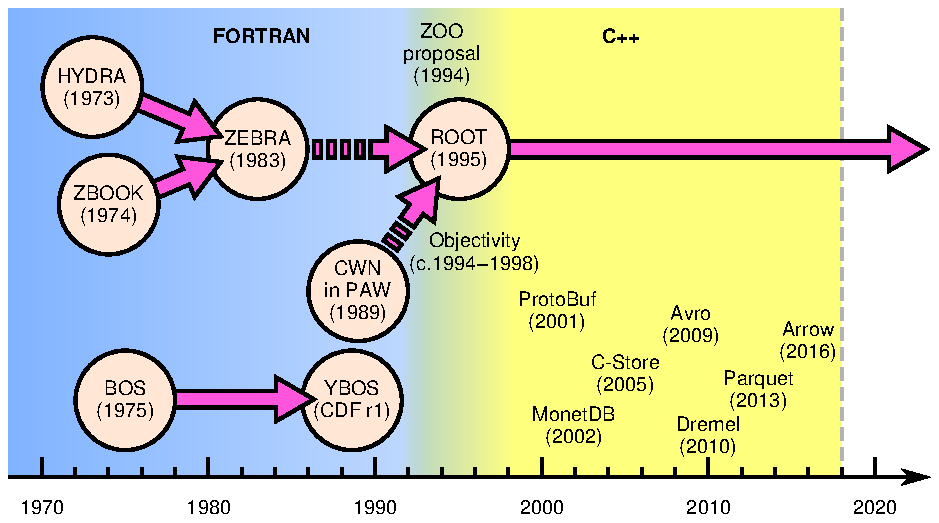
\includegraphics[width=\linewidth]{history.pdf}
\end{frame}

\begin{frame}{The two most significant features, setting HEP apart}
\vspace{0.5 cm}
\begin{columns}[t]
\column{0.5\linewidth}
\textcolor{darkorange}{\bf \underline{\Large Hierarchically nested structures}}

\vspace{0.35 cm}
\textcolor{darkblue}{For example:} event contains jets,

\textcolor{white}{For example:} \hspace{0.5 cm}jets contain tracks,

\textcolor{white}{For example:} \hspace{1 cm}tracks contain hits\ldots

\vspace{0.35 cm}
It's important that the nested objects have variable size, since structs of structs of integers are not {\it really} nested: they compile to constant offsets, just like flat data.

\vspace{0.35 cm}
Fortran (pre-90) didn't have this feature, so physicists had to add it.

\column{0.5\linewidth}
\textcolor{darkorange}{\bf \underline{\Large Columnar representation}}

\vspace{0.35 cm}
\textcolor{darkblue}{For example:} all values of muon~$p_T$ are contiguous in serialized form, followed by all values of muon~$\eta$, all values of muon~$\phi$, and all \#muons per event.

\vspace{0.35 cm}
Thus, you can read muon~$p_T$ without reading jet~$p_T$.

\vspace{0.35 cm}
Easy for flat data: it's just a transpose.

\vspace{0.1 cm}
There are several techniques for solving it in general (hot CS topic in early 2000's).
\end{columns}
\end{frame}

\begin{frame}{20 questions to ask about any file format}
\vspace{0.15 cm}
\small
\begin{columns}
\column{0.5\linewidth}

\begin{block}{Expressiveness}
\vspace{-0.2 cm}
\begin{itemize}\setlength{\itemsep}{-0.05 cm}
\item \textcolor{darkorange}{\bf Hierarchically nested or flat tables?}
\item Has schema (strongly typed) or dynamic?
\item Schema evolution, if applicable?
\item Language agnostic or specific?
\end{itemize}
\end{block}

\vspace{0.5 cm}

\begin{block}{Performance}
\vspace{-0.2 cm}
\begin{itemize}\setlength{\itemsep}{-0.05 cm}
\item \textcolor{darkorange}{\bf Rowwise or columnar?}
\item Compressed/compressible?
\item Robust against bit errors?
\item Serialized/runtime unity?
\end{itemize}
\end{block}

\column{0.5\linewidth}

\begin{block}{Accessibility}
\vspace{-0.2 cm}
\begin{itemize}\setlength{\itemsep}{-0.05 cm}
\item Human readable, binary, or both?
\item Immutable/append only/full database?
\item Parallel readable?
\item Parallel writable?
\item Read streamable?
\item Write streamable?
\item Random accessible?
\item Database-style indexing?
\item RPC protocol?
\end{itemize}
\end{block}

\vspace{-0.2 cm}

\begin{block}{Community}
\vspace{-0.2 cm}
\begin{itemize}\setlength{\itemsep}{-0.05 cm}
\item Has specification?
\item Independent implementations?
\item Size of user base?
\end{itemize}
\end{block}

\end{columns}
\end{frame}

\begin{frame}{Expressiveness: Hierarchically nested or flat tables?}
\vspace{0.5 cm}
Hierarchical nesting could be seen as a special case of graph data, but it's an important special case because hierarchical types may have strongly typed schemas and special contiguity properties, such as rowwise vs.\ columnar.

\vspace{-0.5 cm}

\begin{columns}[t]
\column{0.1\linewidth}
\column{0.4\linewidth}
\begin{center}
Hierarchical

\vspace{0.2 cm}
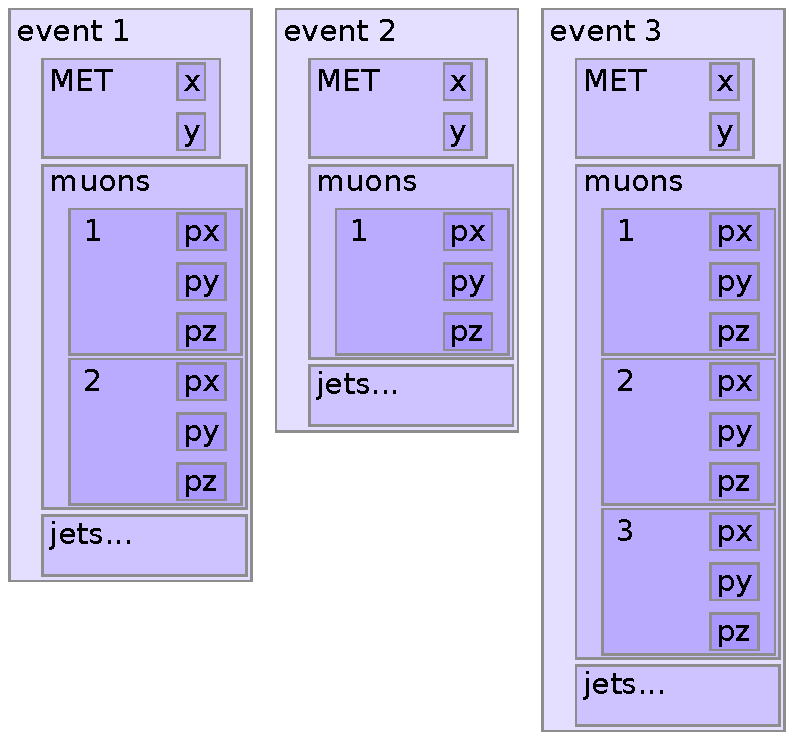
\includegraphics[width=0.7\linewidth]{event-structure.pdf}
\end{center}
\column{0.4\linewidth}
\begin{center}
Flat table

\vspace{0.2 cm}
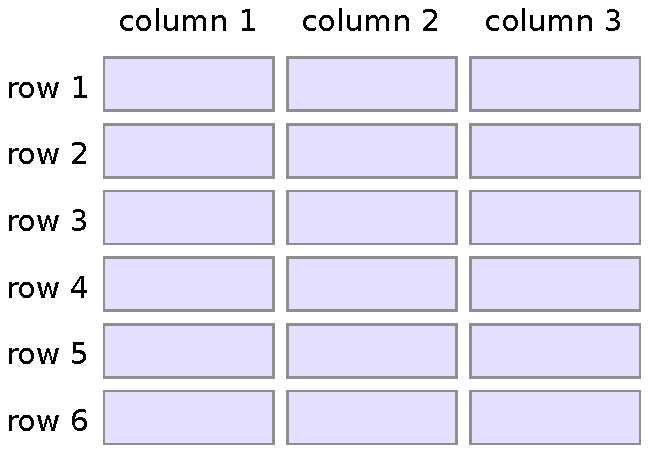
\includegraphics[width=0.7\linewidth]{table-structure.pdf}

\small (conversion to a flat table is {\it lossy!})

\end{center}
\column{0.1\linewidth}
\end{columns}

\vspace{0.25 cm}

\begin{description}
\item[Haves:] ROOT, Parquet, Avro, JSON, XML, and many others\ldots
\item[Have nots:] CSV, SQLite, Numpy, {\it high-performance} HDF5\ldots
\end{description}
\end{frame}

\begin{frame}{Expressiveness: Has schema (strongly typed) or dynamic?}
\vspace{0.5 cm}
Same issue as in programming languages: can we express the data type once for all elements of a collection or do we have to express it separately for each element?

\vfill

\begin{description}
\item[Haves:] ROOT, Parquet, Avro, and many others\ldots
\item[Have nots:] JSON, BSON (binary JSON), MessagePack, and many others\ldots
\end{description}

\vfill

Just as in programming languages, there are arguments for and against schemas, and they're helpful in some situations, harmful in others.

\vfill

In HEP, we know the schema in advance for reasonably large blocks of event data and want the performance advantages of schemas. \textcolor{gray}{Without a schema, every object must be accompanied by type metadata (even if it's just a reference). Repeated field names account for most of JSON and BSON's bloat (it's {\it not} because JSON is text!).}
\end{frame}

\begin{frame}{Expressiveness: Schema evolution, if applicable?}
\vspace{0.5 cm}
\underline{\it If} a schema is used to compile runtime objects, \underline{\it then} a mismatch between an old schema and a new schema can render old data unreadable. Schema evolution is a set of rules to automatically translate data schemas into container objects.

\begin{description}
\item[Haves:] ROOT, ProtoBuf, Thrift, Avro, all in very different ways
\item[Have nots:] Objectivity, Java serialization (without manual effort)\ldots
\item[Inapplicables:] Any schemaless format (e.g.\ JSON) and any format without fixed containers: Google FlatBuffers (runtime indirection), OAMap (JIT)
\end{description}

\vspace{0.25 cm}

Schema evolution isn't a well-defined dichotomy, but a spectrum of techniques filling the continuum between static typing (assert types at the earliest possible time) and dynamic typing (assert types at the latest possible time). ROOT's typing is not strictly ``static'' because it uses a JIT-compiler to compile \href{https://root.cern.ch/root/SchemaEvolution.pdf}{\textcolor{blue}{Streamer Rules}}.

\vspace{0.25 cm}

Generally, we'd like to delay ``hard compiling'' types until {\it after} we've seen the data schema and {\it before} we run over a million events. JIT is a good solution.

\end{frame}

\begin{frame}{Expressiveness: Language agnostic or specific?}
\vspace{0.5 cm}
A serialization format may be specialized to a given language and (eventually) handle every data type in that language. This is true of ROOT, which covers almost all of C++'s types. \textcolor{darkblue}{Good for designing data types for code, rather than serialization.}

\vfill

Alternately, it could define a type system typical of programming languages but not aligned with any one language. These types are then mapped onto each language without a full bijection (e.g.\ all ProtoBuf types can be expressed in C++, but not all C++ types can be expressed in ProtoBuf). \textcolor{darkblue}{Good for cross-language interoperability.}

\vfill

\begin{description}
\item[Agnostic:] ProtoBuf, Thrift, Avro, Parquet, OAMap, SQL schemas
\item[Specific:] ROOT, Cap'n Proto (C++), Pickle (Python), Kryo (Java, in Spark)
\end{description}
\end{frame}

\begin{frame}{Performance: Rowwise or columnar?}
\vspace{0.35 cm}
Columnar representation allows more efficient access to a subset of attributes (the only ones used in an analysis, for instance) because network $\to$ computer, disk $\to$ memory, memory $\to$ CPU, and memory $\to$ co-processor pipelines all cache {\it contiguous bytes.}

\vspace{0.25 cm}
\textcolor{darkblue}{Hierarchically nested example:} {\tt\small vector<vector<pair<char, int>>>}

\vspace{0.25 cm}
\begin{tabular}{r l}
\small logical data & {\tt\scriptsize \textcolor{blue}{[}\textcolor{violet}{[}(\textcolor{darkorange}{a},\textcolor{darkgreen}{1}), (\textcolor{darkorange}{b},\textcolor{darkgreen}{2}), (\textcolor{darkorange}{c},\textcolor{darkgreen}{3}), (\textcolor{darkorange}{d},\textcolor{darkgreen}{4})\textcolor{violet}{]}, \textcolor{violet}{[]}, \textcolor{violet}{[}(\textcolor{darkorange}{e},\textcolor{darkgreen}{5}), (\textcolor{darkorange}{f},\textcolor{darkgreen}{6})\textcolor{violet}{]}\textcolor{blue}{]}, \textcolor{blue}{[]}, \textcolor{blue}{[}\textcolor{violet}{[}(\textcolor{darkorange}{g},\textcolor{darkgreen}{7})\textcolor{violet}{]}\textcolor{blue}{]}\ \textcolor{white}{]}} \\\hline
\small outer stops & {\tt\scriptsize \textcolor{blue}{[\ \ \ \ \ \ \ \ \ \ \ \ \ \ \ \ \ \ \ \ \ \ \ \ \ \ \ \ \ \ \ \ \ \ \ \ \ \ \ \ \ \ \ \ \ \ \ \ 3,\ \ 3,\ \ \ \ \ \ \ \ \ 4]}} \\
\small inner stops & {\tt\scriptsize \textcolor{violet}{[\ \ \ \ \ \ \ \ \ \ \ \ \ \ \ \ \ \ \ \ \ \ \ \ \ \ \ 4,\ \ 4,\ \ \ \ \ \ \ \ \ \ \ \ \ \ 6,\ \ \ \ \ \ \ \ \ \ \ \ \ 7\ ]}} \\
\small 1$^{\mbox{\scriptsize st}}$ attribute & {\tt\scriptsize \textcolor{darkorange}{[\ \ a,\ \ \ \ \ b,\ \ \ \ \ c,\ \ \ \ \ d,\ \ \ \ \ \ \ \ \ \ \ e,\ \ \ \ \ f,\ \ \ \ \ \ \ \ \ \ \ \ \ g\ \ \ \ \ ]}} \\
\small 2$^{\mbox{\scriptsize nd}}$ attribute & {\tt\scriptsize \textcolor{darkgreen}{[\ \ \ \ 1,\ \ \ \ \ 2,\ \ \ \ \ 3,\ \ \ \ \ 4,\ \ \ \ \ \ \ \ \ \ \ 5,\ \ \ \ \ 6,\ \ \ \ \ \ \ \ \ \ \ \ \ 7\ \ \ ]}}
\end{tabular}

\vspace{0.25 cm}
\textcolor{gray}{The ``stops'' column is a running total number of entries at each closing bracket {\it of that level of hierarchy.} The attribute data (leaves of the tree) are stored without boundaries.}

\vspace{0.25 cm}
\begin{description}
\item[Haves:] ROOT (only one level deep), Parquet, ORC (database file), OAMap\ldots
\item[Have nots:] JSON, ProtoBuf, Thrift, Avro, Google FlatBuffers, and many others\ldots
\end{description}
\end{frame}

\begin{frame}{Performance: Compressed/compressible?}
\vspace{0.35 cm}
Of course any file can be compressed, but it sure is convenient if compression is a built-in option. Compression trades read and write throughput for serialized size.

\begin{columns}
\column{0.6\linewidth}
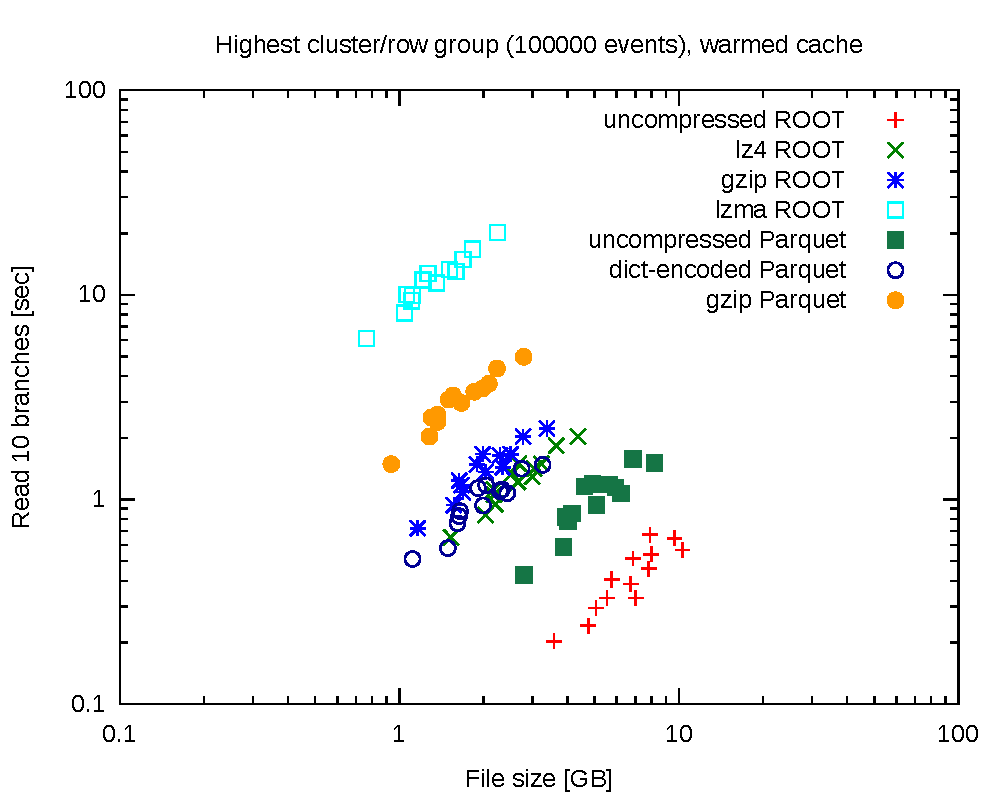
\includegraphics[width=\linewidth]{root-parquet-size-throughput.pdf}
\column{0.4\linewidth}
\small
Some serialization formats skirt the boundary between simple encoding and compression. Parquet {\it with compression turned off} results in \underline{smaller}, \underline{slower} files than ROOT {\it with lz4 compression turned on.}

\vspace{0.25 cm}
\normalsize
\begin{description}
\item[Haves:] ROOT, ProtoBuf, Thrift, Avro, Parquet, HDF5, and many others\ldots
\item[Have nots:] JSON, CSV\ldots
\end{description}
\end{columns}
\end{frame}

\begin{frame}{Performance: Robust aginst bit errors?}
\vspace{0.5 cm}
In large datasets, bit errors can occur. Robustness consists of three questions:
\begin{itemize}
\item Can a bit error be detected, for instance using a CRC?
\item Can a bit error be repaired with replication in the file? \textcolor{gray}{(I've never heard of this.)}
\item If bad data has to be skipped, how much has to be skipped? A page or a \mbox{whole file?\hspace{-1 cm}}
\end{itemize}

\vfill

Since compression increases sensitivity to bit errors (can scramble an entire compression frame), compression formats often have CRC features built in. The question is whether the file format saves CRCs and whether readers check them.

\vfill

\begin{description}
\item[Haves:] ROOT, HDF5, Avro, Parquet, mostly through using the compressor's CRCs. As far as I know, these do not include robustness in object headers, just bulk data.
\item[Have nots:] JSON, CSV\ldots\ Hard to be sure a format with compression doesn't use the CRC.
\end{description}
\end{frame}

\begin{frame}{Performance: Serialized/runtime unity?}
\vspace{0.5 cm}
This is new; increasingly relevant as storage class memory becomes mainstream:

\begin{center}
\begin{minipage}{0.9\linewidth}
\textcolor{red}{Is the byte-representation of serialized data equal to the byte-representation of runtime objects? That is, are data structures zero-copy, zero-conversion?}
\end{minipage}
\end{center}

It allows, for instance, a memory-mapped file to be used directly as runtime data. {\tt\small mmap} (1 system call) is often faster than {\tt\small fread} (many system calls) and deserializing data can be a throughput bottleneck, depending on what you do with it afterward.

\vspace{0.25 cm}

Links: \href{https://www.snia.org/forums/sssi}{\textcolor{blue}{SNIA SSSI}}, \href{https://lwn.net/Articles/717953/}{\textcolor{blue}{DAX direct access}}, \href{https://pmem.io/}{\textcolor{blue}{PMEM development kit}}, \href{http://scitechconnect.elsevier.com/memory-management-unit/}{\textcolor{blue}{MMU mapping}}.

\vspace{0.15 cm}

\begin{description}
\item[Haves:] This is a design goal of the Apache Arrow project, particularly for Spark, Pandas, and R DataFrames. ``Feather'' is memory-mapped Arrow on disk. Apache Drill (SQL) highlights their lack of ``row materialization.'' OAMap with raw data or Arrow as a backend also satisfies this criterion.
\item[Have nots:] Most data formats, including ROOT.
\end{description}
\end{frame}

\begin{frame}{Accessibility: Human readable, binary, or both?}
\vspace{0.5 cm}
From {\it ASDF: A new data format for astronomy} {\small (P.\ Greenfield, M.\ Droettboom, E.\ Bray)}:

\begin{center}
\begin{minipage}{0.9\linewidth}
\scriptsize [HDF5] is an entirely binary format. FITS headers are easily human-readable. Nothing like that is the case for HDF5 files. All inspection of HDF5 files must be done through HDF5 software. With FITS, it is quite possible to inspect the header with very primitive tools. The consequence of this for HDF5 is that the HDF5 toolset must be installed, and its software must be used if one wants to inspect the contents of the HDF5 file in any way.
\end{minipage}
\end{center}

I find it fascinating that human-readability is such an important consideration in astronomy, but HEP never gave it a second thought.

\vspace{0.25 cm}

\textcolor{gray}{Human readable numbers with fewer than 4 or 8 characters may be viewed as a kind of lossy compression, especially when combined with standard compression\ldots}

\vspace{0.25 cm}

\begin{description}
\item[Binary:] ROOT, BSON, and most formats mentioned in this talk
\item[Human:] JSON, CSV, YAML (basis of ASDF)
\item[Both:] FITS, ASDF, YAML (through {\tt\small !!binary}), XML (through {\tt\small CDATA})
\end{description}
\end{frame}

\begin{frame}{Accessibility: Immutable/append only/full database?}
\vspace{0.5 cm}
\end{frame}

\begin{frame}{Accessibility: Parallel readable?}
\vspace{0.5 cm}
\end{frame}

\begin{frame}{Accessibility: Parallel writable?}
\vspace{0.5 cm}
\end{frame}

\begin{frame}{Accessibility: Read streamable?}
\vspace{0.5 cm}
\end{frame}

\begin{frame}{Accessibility: Write streamable?}
\vspace{0.5 cm}
\end{frame}

\begin{frame}{Accessibility: Random accessible?}
\vspace{0.5 cm}
\end{frame}

\begin{frame}{Accessibility: Database-style indexing?}
\vspace{0.5 cm}
\end{frame}

\begin{frame}{Accessibility: RPC protocol?}
\vspace{0.5 cm}
\end{frame}

\begin{frame}{Community: Has specification?}
\vspace{0.5 cm}
\end{frame}

\begin{frame}{Community: Independent implementations?}
\vspace{0.5 cm}
\end{frame}

\begin{frame}{Community: Size of user base?}
\vspace{0.5 cm}
\end{frame}

\end{document}
